\section{Coulomb-nuclear interference}

%----------------------------------------------------------------------------------------------------

\subsection{Theoretical framework}
\label{sec:cni_framework}

Elastic scattering of protons is a process caused by the strong and electromagnetic interactions -- the weak interaction can be neglected since its carriers are heavy compared to the small momentum-transfers typical for elastic scattering. In this context, the strong interaction is traditionally called nuclear and the electromagnetic called Coulomb. In quantum-theory description, each of the interactions generates a scattering amplitude, nuclear ${\cal A}^{\rm N}$ and Coulomb ${\cal A}^{\rm C}$. Moreover, since the interactions act simultaneously, their interference needs to be taken into account, too. The Coulomb amplitude can be calculated from QED (e.g.~section 3.2 in \cite{block06}), using empirical electric and magnetic form factors of the proton (e.g.~\cite{puckett10}). It can be shown (e.g.~section 1.3.1 in \cite{jan_thesis}) that, at low $|t|$, the effect of both form factors can be describe by a single function ${\cal F}$. Since the Coulomb amplitude is known, the Coulomb-nuclear interference (CNI) exposes the phase of the nuclear amplitude, otherwise not directly observable in differential cross-section. \todo{why phase interesting?} \todo{introduce: coulomb-interference formula}


%----------------------------------------------------------------------------------------------------
\subsubsection{Nuclear amplitude}

Since the nuclear amplitude can not be currently calculated from first principles, its mathematical description shall be discussed.

The {\bf modulus} is closely related to the differential cross-section and thus strongly constrained by experimental observations. Following especially \cite{8tev-90m}, the modulus will be parametrised:
\begin{equation}
\label{eq:nuc mod}
| {\cal A}^{\rm N}(t) | = a \exp\left( \sum\limits_{n}^{N_b} b_n t^n \right)\ ,
\end{equation}
\todo{for $|t| < 0.2$, what about higher $|t|$'s?}\\
where $N_b$ gives the number of free parameters in the exponent. This implicitly extends the exponential-like behaviour to the regions where the (pure nuclear) cross-section can not be observed. Although there is no rigorous justification, and therefore it stands as an assumption, it is compatible with many theoretical models.

For the {\bf phase} of the nuclear amplitude, there is little experimental guidance and therefore several theory-motivated choices will be assumed and tested.

\begin{itemize}

% ***
\item A {\it constant phase} is obviously the simplest choice:

\begin{equation}
\label{eq:nuc phase const}
\arg {\cal A}^{\rm N}(t) = \hbox{const.}
\end{equation}

% ***
\item The parametrisation by {\em Bailly et al.}~\cite{bailly87} implements the main features of many theoretical models -- almost imaginary amplitude in the forward direction while purely real in the (first) diffraction dip:
\begin{equation}
\label{eq:nuc phase std}
	%\arg {\cal A}^{\rm N}(t) = {\pi\over 2} - \arctan {\rho_0\over 1 - {t\over t_{\rm d}}},\ \rho_0 = {1\over \tan p_0}
	\arg {\cal A}^{\rm N}(t) = \arctan \left[ \tan p_0 \left(1 - {t\over t_{\rm d}} \right) \right]\ ,
\end{equation}
where $p_0$ determines the phase value at $t=0$ and $t_{\rm d} \approx -0.53\un{GeV^2}$ gives the position of the diffractive minimum at $8\un{TeV}$ (preliminary result from $90\un{m}$ data).

% ***
\item \todo{add standard phase ??}

% ***
\item The {\it peripheral phase} \cite{kl94} \todo{newer ref - if we ever get one} provides an alternative to the above descriptions. Its parametrisation

\todo{update values, range?}

\begin{equation}
\label{eq:nuc phase per}
\arg {\cal A}^{\rm N}(t) = p_0 - A \exp\left[ \kappa \left( \log {t\over t_{\rm m}} - {t\over t_{\rm m}} + 1 \right) \right]
\end{equation}
results in a peak with at $t_{\rm m} \approx -0.310\un{GeV^2}$, amplitude $A \approx 5.53$ and width controlled by $\kappa \approx 4.01$.

\end{itemize}

It should be noted that the phase has decisive influence on the amplitude behaviour in the space of impact parameter, $b$, see e.g.~section 3 in \cite{klk02}. It can be quantified by evaluating the root-mean-squares (RMS) of $b$ for elastic and inelastic collisions. The constant and standard phase lead to elastic collisions more central (smaller RMS) than the inelastic ones. The peripheral phase can yield a description with the opposite hierarchy, which is argued more natural by some authors (e.g.~section 4 in \cite{kl96}).

%----------------------------------------------------------------------------------------------------
\subsubsection{Coulomb-nuclear interference formulae}

The {\bf simplified West-Yennie formula (SWY)} \cite{wy68} is derived in the framework of perturbative QFT by evaluating the lowest-order Feynman diagrams that comprise both nuclear and Coulomb interactions. In this approach, the interference is reduced to an additional phase between the Coulomb and nuclear amplitudes. Moreover, several approximations were used in the derivation. First, in order to avoid integrating over off-mass-shell contributions to the nuclear amplitude (purely known), very slow variation of the nuclear amplitude phase was assumed: $\arg {\cal A}^{\rm N} \approx \hbox{const}$. Then, in order to obtain a closed-form expression, the exponential slope of the nuclear modulus
\begin{equation}
B^{\rm N}(t) = {\d \log |{\cal A}^{\rm N}|^2 \over \d t}
\end{equation}
was assumed constant. The original formula did not contain the electromagnetic form factor ${\cal F}$, it was added later by hand:
\begin{equation}
\label{eq:int swy}
	\begin{aligned}
		{\d\sigma\over \d t}^{\rm C+N} &= {\pi (\hbar c)^2 \over s p^2} \left | {\alpha s\over t} {\cal F}^2 \e^{\I\alpha \Phi(t)} + {\cal A}^{\rm N} \right |^2\ ,\cr
		\Phi(t) &= - \left( \log {B |t|\over 2} + \gamma \right)\ ,\cr
	\end{aligned}
\end{equation}
where $\gamma \doteq 0.577$ is the Euler constant. Despite the many limitations, the formula has extensively been used in past data analyses. For backward-comparison reasons we consider it also in this report.

The {\bf Kundr\' at-Lokaj\' i\v cek formula (KL)} \cite{kl94} was derived in an impact parameter formalism and it is based on the additivity of eikonals. The derivation poses no limitations on nuclear amplitude and the formula naturally incorporates the electromagnetic form-factor. In this treatment, the interference effect goes beyond a single phase, the $\Psi$ quantity is complex, in general:
\begin{equation}
\label{eq:int kl}
	\begin{aligned}
		{\d\sigma\over \d t}^{\rm C+N} &= {\pi (\hbar c)^2 \over s p^2} \left | {\alpha s\over t} {\cal F}^2 + {\cal A}^{\rm N} \e^{\I\alpha \Psi(t)} \right |^2\ ,\cr
		\Psi(t) &= 
			- \int \d t'\, \log {t'\over t} {\d\phantom{t'}\over \d t'} {\cal F}^2(t') \cr
		&\phantom{=} + \int \d t' \left( {{\cal A}^{\rm N}(t') \over {\cal A}^{\rm N}(t)} - 1 \right) { I(t, t')\over 2\pi }
			\ ,\cr
		I(t, t') &= \int_0^{2\pi} \d\phi\ {{\cal F}^2(t'')\over t''}\ , \cr
		t'' &= t + t' + 2\sqrt{t\, t'} \cos\phi\ ,\cr
	\end{aligned}
\end{equation}
where the $t$ integrations go over the entire kinematically allowed region.

Calculation engine \cite{elegent}, using form-factor of Puckett et al.~\cite{puckett10}

%----------------------------------------------------------------------------------------------------
\subsection{Data analysis}
\label{sec:cni_anal}

\> nuclear modulus: anchored to $90\un{m}$ data at $|t| > 0.2\un{GeV^2}$ for stability of integrations in \ref{eq:int kl}

\> with the presented data not possible to distinguish between different models/assumptions above $\Rightarrow$ {\bf conditional} determination of parameters of interest
\>> $\rho$
\>> total cross-section and $B$ with Coulomb separated
\>> RMS b elastic, inelastic


Generalised $\chi^2$ fits:
\begin{equation}
\label{eq:chi sq}
	\chi^2 = \vec\Delta^\T \mat{V}^{-1} \vec\Delta\ ,
\end{equation}
where $\vec\Delta$ represents vector of differences in $\d\sigma/\d t$ between fit and measurement for each point and $\mat{V}$ stands for the measurement covariance matrix. The covariance matrix receives three contributions: from statistical uncertainties (diagonal), from systematic uncertainties other than normalisation (independent between $90$ and $1000\un{m}$ data) and from normalisation uncertainty (common source for both datasets).

\> extensive MC tests (input: phenomenological models as well as data fits)
\>> check for bias: only small
\>> understanding/evaluation of the method response to statistical and systematic uncertainties

\> results ($\rho$, $\sigma_{\rm tot}$, $B^{\rm N}(0)$, ...)
\>> for the model choices above -- keeping phase parameters fixed at their central values from Vojt\v ech
\>> for peripheral-phase parameters being varied within their uncertainties $\Rightarrow$ uncertainty band
\>> illustrative decomposition of uncertainties from MC

\> question: do we want to present a single-value result for $\rho$ (combined from fits under different models) ??

\> discuss the new value of $\sigma_{\rm tot}$ in comparison to our previous measurement \cite{prl111}; values compatible; remind in what is the new measurement better ??

\> reference to Fig.~\ref{fig:rho_s}

\> RMS of b for the final fits??

\begin{figure*}
\begin{center}
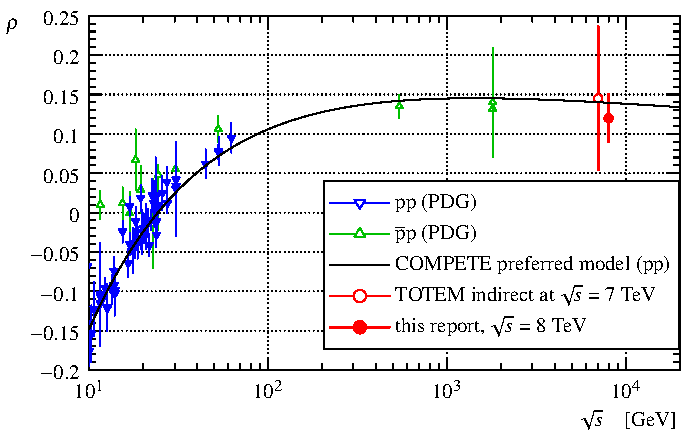
\includegraphics[width=16cm]{fig/rho_s.pdf}
\vskip-3mm
\caption{$\rho$ as a function of $s$.}
\label{fig:rho_s}
\end{center}
\end{figure*}

\> figure for $\sigma_{\rm tot}$ result ??
